\documentclass[12pt]{article}

\usepackage[T1]{fontenc}
\usepackage[utf8]{inputenc}
\usepackage[russian]{babel}

% page margin
\usepackage[top=2cm, bottom=2cm, left=2cm, right=2cm]{geometry}

% AMS packages
\usepackage{amsmath}
\usepackage{amssymb}
\usepackage{amsfonts}
\usepackage{amsthm}

\usepackage{graphicx}

\usepackage{fancyhdr}
\pagestyle{fancy}
% modifying page layout using fancyhdr
\fancyhf{}
\renewcommand{\sectionmark}[1]{\markright{\thesection\ #1}}
\renewcommand{\subsectionmark}[1]{\markright{\thesubsection\ #1}}

\rhead{\fancyplain{}{\rightmark }}
\cfoot{\fancyplain{}{\thepage }}

\usepackage{titlesec}
\titleformat{\section}{\bfseries}{\thesection.}{1em}{}
\titleformat{\subsection}{\normalfont\itshape\bfseries}{\thesubsection.}{0.5em}{}

\newcommand{\mf}{\mathbf}

\newcommand{\lb}{\left(}
\newcommand{\rb}{\right)}

\newcommand{\mH}{\mathcal{H}}

\newcommand{\intl}{\int\limits}
\newcommand{\idotsintl}{\idotsint\limits}

\begin{document}

\section*{Расчет константы равновесия K$_p$(N$_2-$N$_2$)}

Первый вариант. По формуле из статьи I. Buryak, A. Vigasin (2015):
\begin{gather}
	K_p^{bound} = \lb R T \rb^{-1} \frac{N_0}{2s} \idotsintl_{U \lb R, \Omega \rb < 0} \exp \lb - \frac{U}{kT} \rb \frac{ \gamma \lb \frac{7}{2}, - \frac{U}{kT} \rb}{\Gamma \lb \frac{7}{2} \rb } R^2 d R \, d \Omega = \hspace{5cm} \notag \\
	\hspace{5cm} = \frac{N_0}{4 R T} \idotsintl_{U \lb R, \theta_1, \theta_2, \varphi \rb < 0} \exp \lb - \frac{U}{k T} \rb \frac{ \gamma \lb \frac{7}{2}, - \frac{U}{k T} \rb}{\Gamma \lb \frac{7}{2} \rb} R^2 \sin \theta_1 \sin \theta_2 \, dR \, d \theta_1 \, d \theta_2 \, d \varphi \notag
\end{gather}

Второй вариант. Интегрирование по полному фазовому пространству. \par
Классическая сумма по состояниям связанного димера представляет собой следующий фазовый интеграл
\begin{gather}
		Q_{bound}^{pair} = \frac{1}{h^{10}} \intl_{H - \displaystyle \frac{P_{cm}^2}{2M} < 0} \exp \lb - \frac{H}{k T} \rb d x_{cm} \, d y_{cm} \, d z_{cm} \, d P_x \, d P_y \, d P_z \, d q_i \, d p_i, \label{full1} 
\end{gather}

где $q_i, p_i$ -- набор внутримолекулярных координат и импульсов, $H$ -- гамильтониан, записанный в лабораторной системе координат, $\mf{R} = \lb x_{cm}, y_{cm}, z_{cm} \rb$, $\mf{P}_R = \lb P_x, P_y, P_z \rb$ -- векторы координат и импульсов центра масс, а $M$ -- его масса. \par
Гамильтониан $H$ в лабораторной системе координат отличается от гамильтонианом $\mH$ в молекулярной системе координат на кинетическую энергию центра масс
\begin{gather}
		H = \mH + \frac{P_{cm}^2}{2 M} \notag
\end{gather}

Интегрирование по координатам центра масс в \eqref{full1} дает трансляционную статсумму
\begin{gather}
	\lb Q_{bound}^{pair} \rb_{tr} = \lb \frac{2 \pi M k T}{h^2} \rb^\frac{3}{2} V \notag
\end{gather}

Интегрирование в $\eqref{full1}$ в том числе производится по эйлеровым углам и импульсам. Т.к. подынтегральное выражение не зависит от эйлеровых углов, то интегрирование по ним сводится к умножению на величину отрезка интегрирования. Осуществим замену от эйлеровых импульсов к компонентам углового момента. Представим вышесказанное в виде виде интегрального соотношения
\begin{gather}
	\intl_{0}^{2 \pi} d \varphi \intl_{0}^{\pi} d \theta \intl_{0}^{2 \pi} d \psi \int d p_\varphi \int d p_\theta \int d p_\psi = 8 \pi^2 \int d J_x \int d J_y \int d J_z \notag
\end{gather}

Однако в случае N$_2-$N$_2$, как и в случае CO$_2-$Ar, вращение на углы $\psi$, большие $\pi$, не приводит к новым состояниям системы из-за симметричности обоих молекулярных фрагментов. Поэтому интегральное соотношение сводится к следующему
\begin{gather}
	\intl_{0}^{2 \pi} d \varphi \intl_{0}^{\pi} d \theta \intl_{0}^{\pi} d \psi \int d p_\varphi \int d p_\theta \int d p_\psi = 4 \pi^2 \int d J_x \int d J_y \int d J_z \notag
\end{gather}

Итак, с учетом описанной замены переменных статсумма связанного димера $\eqref{full1}$ принимает вид
\begin{gather}
	Q_{bound}^{pair} = \lb Q_{bound}^{pair} \rb_{tr} \frac{4 \pi^2}{h^7} \idotsintl_{\mH < 0} \exp \lb - \frac{\mH}{k T} \rb dR \, d p_R \, d \theta_1 \, d p_\theta_1 \, d \theta_2 \, d p_\theta_2 \, d \varphi \, d p_\varphi \, d J_x \, d J_y \, d J_z \notag 
\end{gather}

Константа равновесия вычислялась по следующему соотношению
\begin{gather}
		K_p = \frac{N_A}{p} \frac{Q_{bound}^{pair}}{Q_{N_2}^2}, \quad Q_{N_2} = Q_{N_2}^{tr} Q_{N_2}^{rot} = \lb \frac{2 \pi m_{N_2} R T}{h^2} \rb^\frac{3}{2} V \, \frac{4 \pi^2 k T}{h^2} \mu_1 l_{N_2}^2, \quad \mu_1 = \frac{1}{2} m_{N_2} \notag  
\end{gather}

\begin{figure}[!ht]
	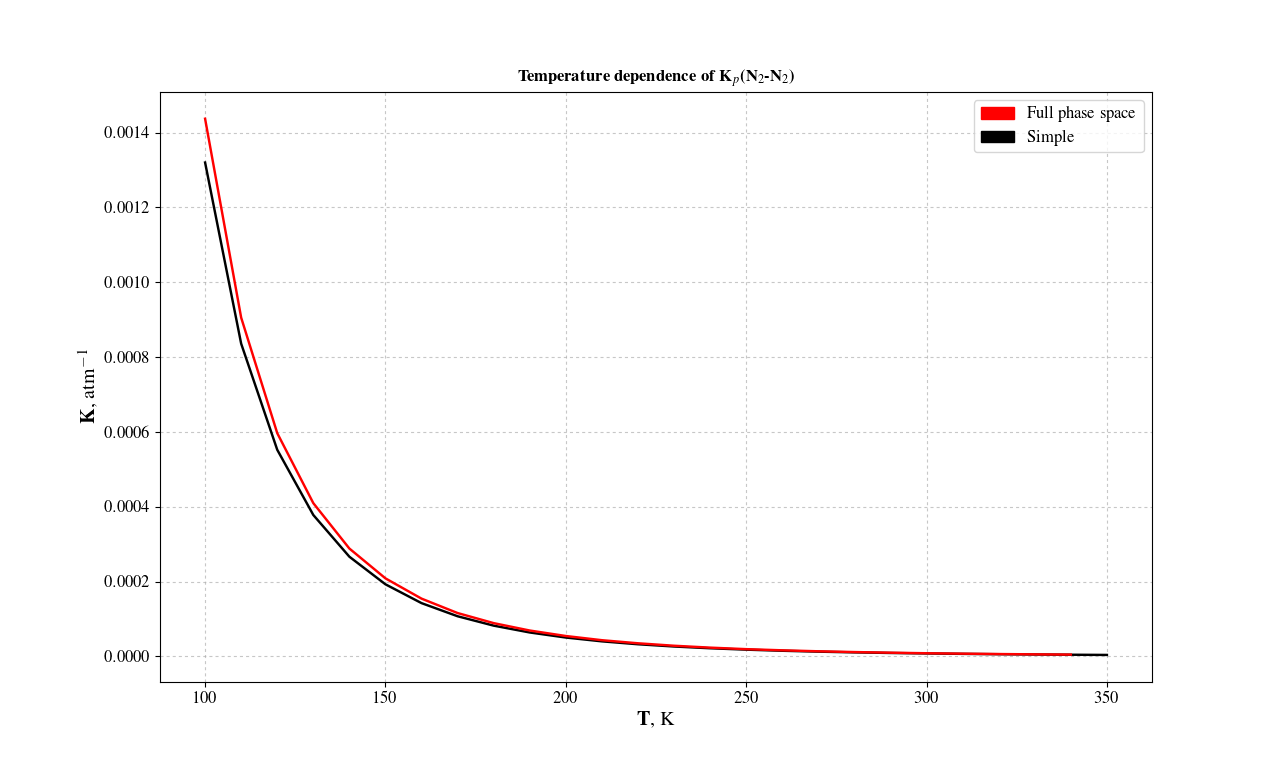
\includegraphics[width = \linewidth]{../results/plot.png}
	\caption{Температурные зависимости констант равновесия, полученных двумя способами}
\end{figure}

\end{document}
